\chapter{RHuBarb: Speeding up Edge-Centric Processing using Recursive Hilbert Blocking}
\label{ch:Rhubarb}

% In Chapter \ref{ch:CaseStudy}, we illustrated the performance improvement that is gained by traversing the edges of the graph using the Hilbert Curve for a variety of graph datasets and orderings.
% This motivated our design and implementation of the Parallel SlashBurn algorithm. 
% However, our case-study was performed using a \textit{single-threaded} PageRank implementation, while all modern multithreaded GPS try to efficiently use all available cores when computing graph analytics for the purposes of scalability and speed. 
% This naturally leads to the following question:
% \begin{enumerate}
%     \item Can we efficiently parallelize the execution of edge-centric algorithms that order the edges using the Hilbert curve while maintaining the cache locality benefit seen using a single thread?
%     % gained by a single-threaded traversal of the same space filling curve?

% \end{enumerate}

In Chapter \ref{ch:CaseStudy}, we showed how using the Hilbert Curve to traverse the edges of a graph can improve performance for various datasets and vertex orderings. This led us to develop the Parallel SlashBurn algorithm. However, our case study only used a single-threaded PageRank implementation. Modern multithreaded Graph Processing Systems try to use all available cores to improve scalability and speed. This raises the question: can we effectively parallelize edge-centric algorithms that use the Hilbert curve to order edges, while still benefiting from the improved cache locality that is obtained by traversing the Hilbert Curve using a single thread?


\textbf{RHuBarb} is our solution to this question. Rhubarb is an edge reordering and blocking technique that uses \textbf{R}ecursive \textbf{H}ilbert \textbf{B}locking, and is geared towards parallel computation of edge-centric algorithms.\\
In this chapter we describe the main challenges that we encountered in our parallelization of the Hilbert Curve:
\begin{enumerate}
    \item Ensuring safe writes from multiple threads to vertex data.
          % \begin{itemize}
    \item Overcoming inefficiencies in OpenMP \cite{openmp} array reductions.
          % \end{itemize}
    \item Using a thread schedule and work assignment that maintains an even work distribution and  locality of read/write access to shared arrays of vertex data.
\end{enumerate}

Then, we describe the techniques we used and designed to address these concerns. Namely:
\begin{enumerate}
    \item Spray: Sparse Reductions of Arrays in OpenMP \cite{spray}, and
    \item Recursive Hilbert Blocking.

\end{enumerate}

% Finally, we describe our implementation of three edge-centric algorithms: PageRank, Connected Components, and Collaborative Filtering using Rhubarb.



\section{Issues Arising in Parallel Edge-Centric Computation}
A simple way to parallelize edge-centric computation using the Hilbert Space Filling Curve would be to split the graph's adjacency matrix into equally sized quadrants and to assign each thread the edges in each quadrant. However, two issues arise from this na\"{\i}ve  parallelization approach:


\begin{itemize}
    \item [\textbf{Challenge 1}] - \textbf{Potential write contention}:
          % Threads may attempt to concurrently update the same 
          % destination vertex data. For example, in the figure, if Thread 1 processes the edge $(0, 1)$ at the same time as when Thread 2 processes the edge $(2, 1)$, the updates to destination vertex $1$ may be clobbered. 
          % If multiple threads concurrently update the same destination vertex data, there may be conflicts resulting in clobbered updates. For example, if Thread 1 processes the edge $(0, 1)$ at the same time as Thread 2 processes the edge $(2, 1)$, the updates to destination vertex $1$ may be lost.
          If multiple threads concurrently update the same destination vertex's data, there
          may be conflicts resulting in clobbered updates. We illustrate such a conflict in Figure \ref{fig:hilbert_update_issue}: if Thread 1 processes the edge $(0, 1)$ at the same time as Thread 2 processes the edge $(2, 1)$, the updates to destination vertex $1$ may be lost.
    \item [\textbf{Challenge 2}] - \textbf{Uneven distribution of work between threads}: Splitting up the
          adjacency matrix into quadrants with equal side-length can lead to an uneven
          distribution of edges between threads. Since quadrants act as the base unit of work which is assigned to threads, and there is no guarantee that the edges are distributed evenly amongst the quadrants, this may cause an uneven work distribution between threads, resulting in some threads finishing their work earlier than others (i.e., stagglers). This issue is illustrated in Figure
          \ref{fig:uneven_work}.
\end{itemize}

\begin{figure}[!htb]
    % \centering
    % 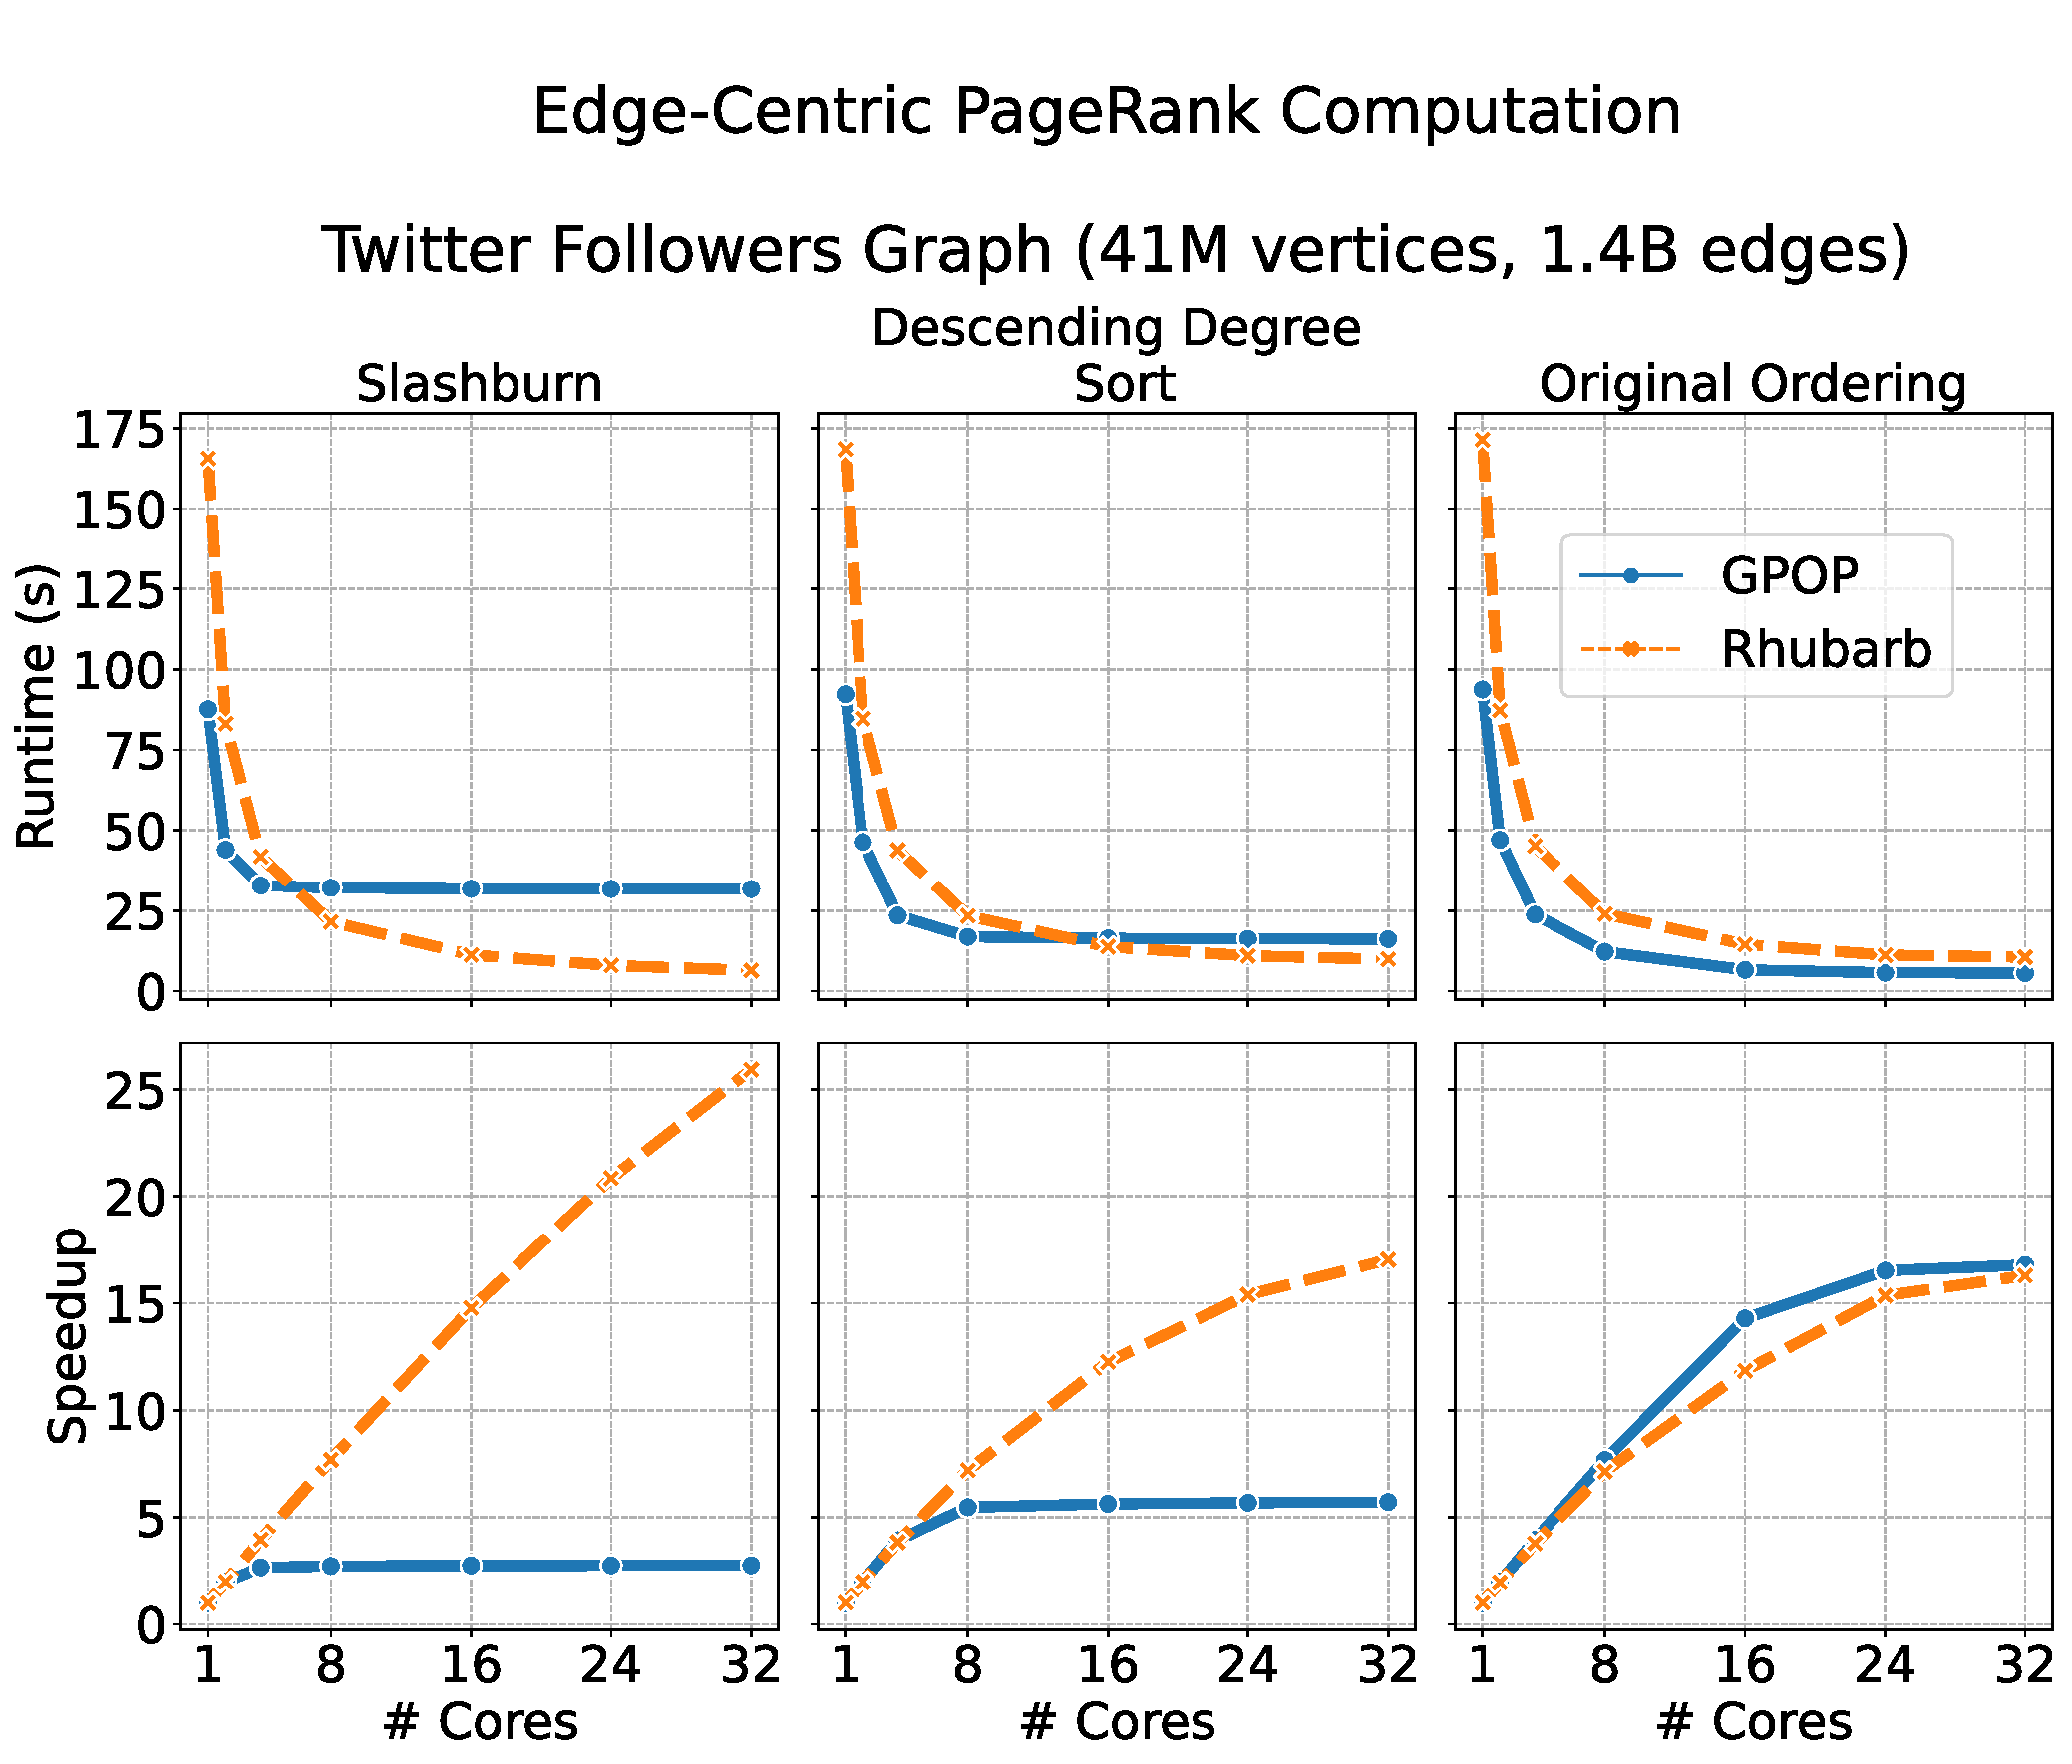
\includegraphics[width=5in]{plots/eval/twitter-sample.pdf}
    % \includesvg[width=6in]{../ipe_plots/hilbert_write_contention.svg}
    \includesvg[width=6in]{./ipe_plots/hilbert_write_contention.svg}

    % Since the Hilbert Space Filling Curve is defined recursively, it follows that 
    % parallelizing of edge-centric computation of the edges that lie on the Hilbert curve could be done by splitting the graph's adjacency matrix into equally sized quadrants. We can then assign each thread the edges that lie in each quadrant.
    % Two issues arise from this parallelization:
    \caption{Potential write contention due to parallel processing of edges using the Hilbert curve. (Figure adapted from \cite{gao2017high}).}
    \label{fig:hilbert_update_issue}   % label should change
\end{figure}
\newpage
\begin{figure}[!htb]
    \centering
    \subfloat[Adjacency Matrix of the CiaoDVD Social Network graph \cite{konect}. A marked blue pixel in the $(i, j)^{\text{th}}$ coordinates corresponds to the existence of an edge $(i, j)$ in the graph.
        % The plot shows the graph's original vertex ID assignment. 
        The graph's edges have been partitioned into quadrants of size $1024\times 1024$.]{
        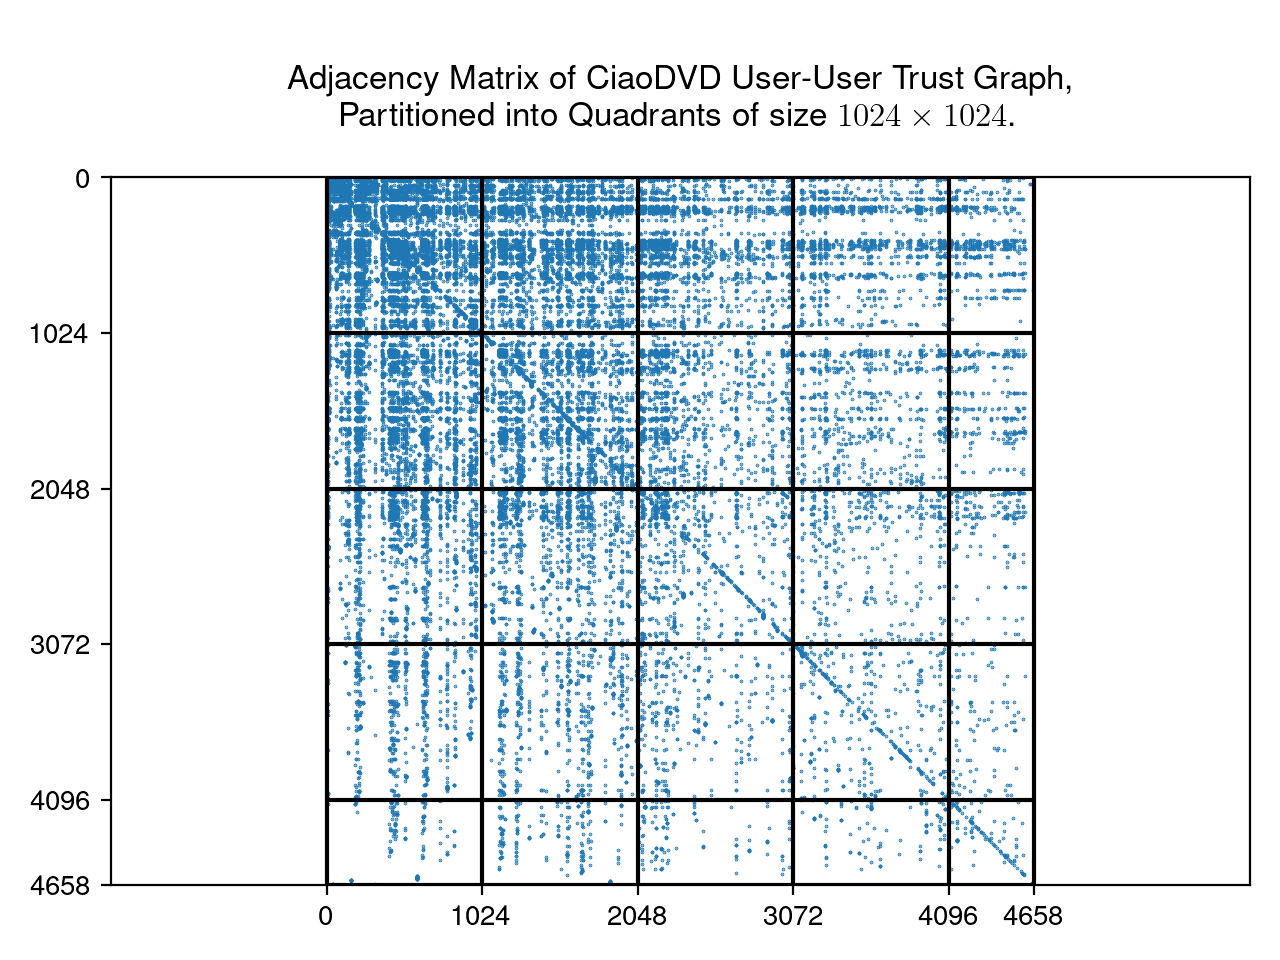
\includegraphics[width=4in]{figures/work_dist_adj_mat.png}
        \label{fig:work_dist_fig}
    }\qquad
    \subfloat[Number of edges per quadrant in Figure \ref{fig:work_dist_fig}.]{
        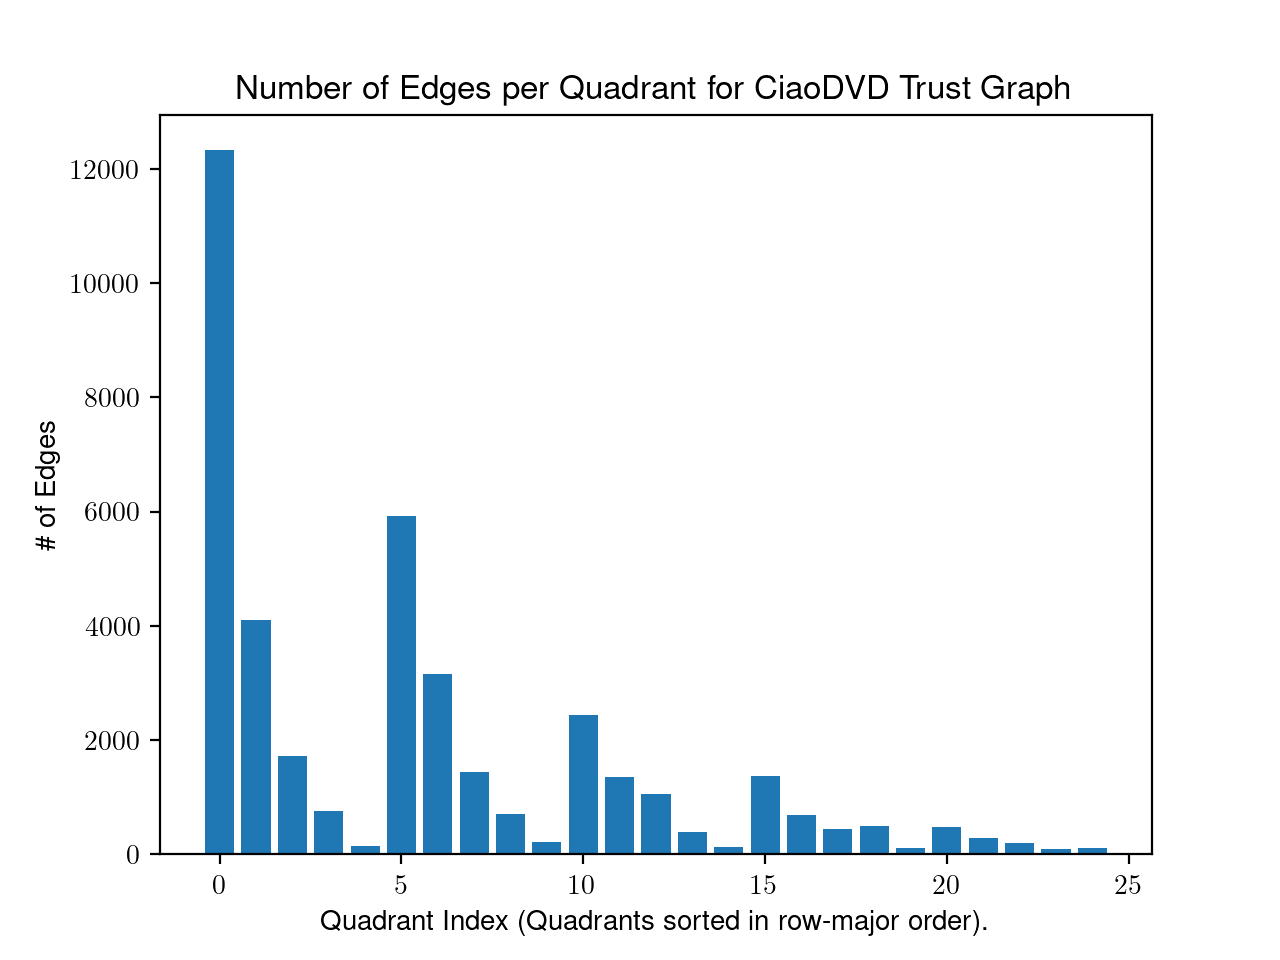
\includegraphics[width=4in]{figures/work_dist.png}
        \label{3figs-c}
    }
    \caption{Uneven distribution of edges due to quadrant partitioning.}
    \label{fig:uneven_work}
\end{figure}
\newpage
\section{Addressing Challenge 1: Efficient Sparse Reductions of Arrays using Spray}
% \AT{
%     I'll start this section by discussing the traditional (and inefficient) way that parallel reductions of
%     arrays was done in OpenMP \cite{openmp}, which is also how previous work (\cite{cagra})
%     attempted to parallelize edge-centric computation using the Hilbert curve. This is where each thread gets its own private copy of the vertex data array, and all thread-private data is merged (e.g. summed) at the end of each iteration. This will motivate my use of Spray \cite{spray} which avoids the allocation of large thread-private arrays by using Block Reductions, and is thus able to scale.
% }
% This chapter addresses Challenge 1: Efficient Sparse Reductions of Arrays using Spray. 
The traditional method of parallel reductions of arrays in OpenMP \cite{openmp} and previous attempts to parallelize edge-centric computation using the Hilbert curve \cite{cagra} have been inefficient: each thread maintained its own private copy of the vertex data array, and all thread-private data was merged (i.e. summed) at the end of each iteration. In this section, we will discuss an alternative approach that uses Block Reductions with Spray \cite{spray}, which avoids the allocation of large thread-private arrays and enables scalability.

\section{Addressing Challenge 2: Recursive Hilbert Blocking}
% \AT{
%     Recursive Hilbert Blocking and Greedy Merging work together to ensure a balanced distribution of edges between blocks. I'll describe the Recursive Hilbert Blocking algorithm and provide pseudo-code for each subsection. Together, all the pseudocode procedures will make up the entire preprocessing algorithm.
%     The final subsection will describe the use of OpenMP dynamic scheduling and chunking. This means that once the final block array has been computed, we dynamically assign groups of consecutive blocks (determined by a hyperparameter, $c$, chunksize), to ensure that the read/write accesses a core makes when iterating over its assigned blocks is limited to a contiguous and cacheable vertex ID range.
% }

This section introduces Recursive Hilbert Blocking, which is an edge reordering and blocking technique 
% used in conjunction with Greedy Merging to 
that ensures a balanced distribution of edges between blocks. In the first two sections we will describe the Recursive Hilbert Blocking algorithm and provide pseudo-code for each of its procedures. Finally, we will discuss the use of OpenMP scheduling and chunking to dynamically assign groups of consecutive blocks (determined by a hyperparameter, $c$, chunksize). This limits the read/write accesses that a core makes when iterating over its assigned blocks to a contiguous and cacheable vertex ID range.

\subsection{Parallel Divide-and-Conquer using OpenMP \texttt{tasks}}
\subsection{Parallel Greedy Merging of Blocks}
\subsection{OpenMP Dynamic Scheduling}

% \section{Edge-Centric Algorithms in Rhubarb}
% In this section we describe how we implemented three Edge-Centric algorithms in Rhubarb. 
% % \AT{dynamic scheduling in OpenMP, and grouping of consecutive blocks in the Hilbert curve.}
% \subsection{PageRank}
% \subsection{Connected Components}
% \subsection{Collaborative Filtering}
% \begin{figure}[!htb]
%     \begin{subfigure}{.5\textwidth}
%       \centering
%       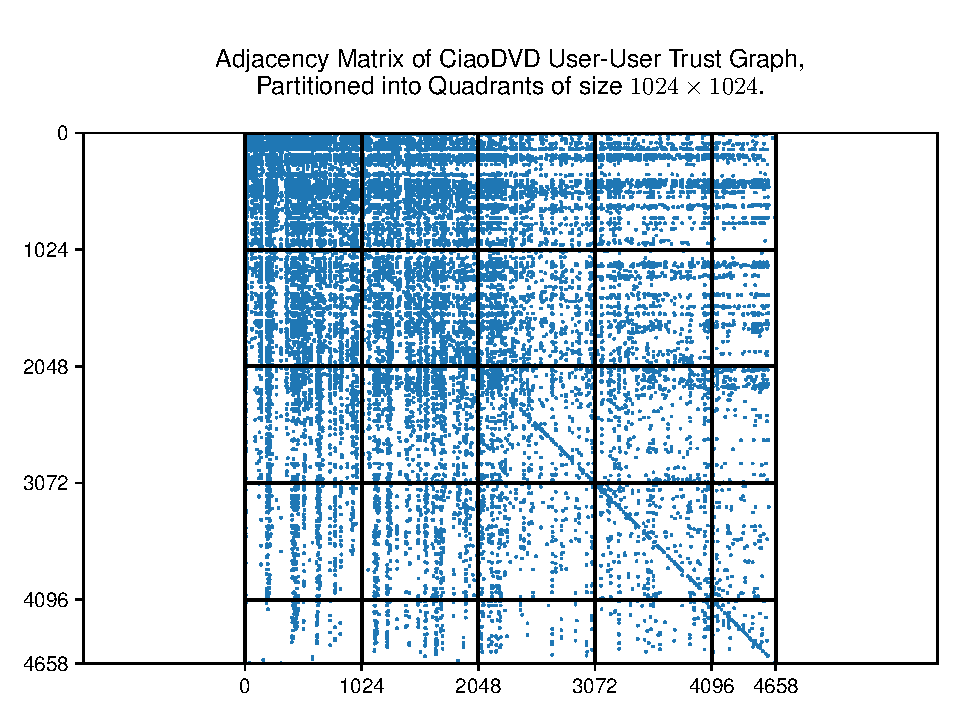
\includegraphics[width=.8\linewidth]{figures/work_dist_adj_mat.pdf}
%       \caption{1a}
%       \label{fig:sfig1}
%     \end{subfigure}%
%     \begin{subfigure}{.5\textwidth}
%       \centering
%       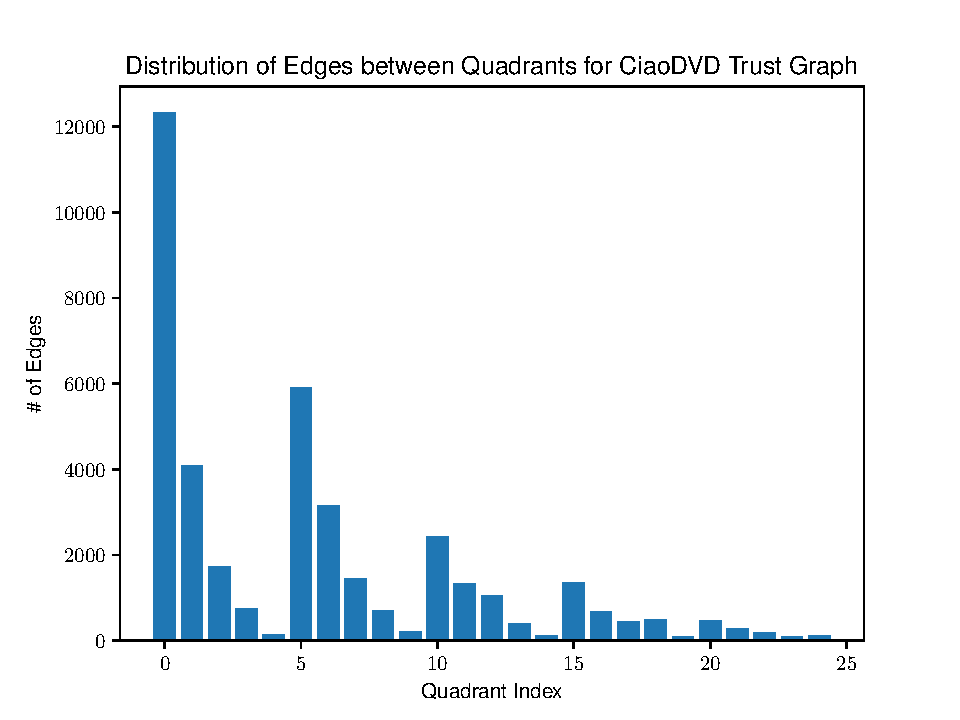
\includegraphics[width=.8\linewidth]{figures/work_dist.pdf}
%       \caption{1b}
%       \label{fig:sfig2}
%     \end{subfigure}
%     \caption{plots of....}
%     \label{fig:uneven_work}
%     \end{figure}

% \algnewcommand{\LineComment}[1]{\State \(\triangleright\) #1}
% \begin{algorithm}
%     \hspace*{\algorithmicindent} \textbf{Input}\\
%     \hspace*{\algorithmicindent}$C$: Graph stored in CSR format \\
%     \hspace*{\algorithmicindent}$C$.index: an $|n|$ array \\
%     \hspace*{\algorithmicindent}$u_0, u_1$: start and end source vertices\\
%     \hspace*{\algorithmicindent}$v_0, v_1$: start and end destination vertices\\
%     \hspace*{\algorithmicindent} \textbf{Output} \\
%     \hspace*{\algorithmicindent} The number of edges in Graph $C$ that lie within the
%     quadrant $[u_0:u_1, v_0:v_1]$
%     \begin{algorithmic}[1]
%         % \LineComment{Given the quadrant specified by the bounds }
%       \Function{n\_edges}{$C, u_0, u_1, v_0, v_1$}  
%     %   \Comment{this is a comment}
%       \State nnz = 0
%       \For{$u$ in range($u0, u1$):}
%       \State neigh\_u\_start = $C$.index[$u$]
%       \State neigh\_u\_end = $C$.index[$u + 1$] \Comment{Start, Endpoint of $u$'s neighbourhood}
%     \LineComment{Binary search to find the index of the first and last out-neighbour }
%     \LineComment{of $u$ that lies in this quadrant}
%       \State first\_idx\_in\_q = lower\_bound($C$.neighbours)
%       \State last\_idx\_in\_q
%         \EndFor 
%       \EndFunction
%     \end{algorithmic}
%   \end{algorithm}